\documentclass[conference, 12pt, onecolumn]{IEEEtran}
\usepackage{cite}
\usepackage{graphicx}
\usepackage{textcomp}
\usepackage{xcolor}
\usepackage{caption}
\usepackage{listings}
\lstset{
  basicstyle=\ttfamily,
  columns=fullflexible,
  numbers=left,
  frame=single,
  breaklines=true,
  postbreak=\mbox{\textcolor{red}{$\hookrightarrow$}\space},
}
\PassOptionsToPackage{hyphens}{url}\usepackage{hyperref}

\date{}

\begin{document}
\title{Maskit: COVID-19 Resiliency through Computer Vision and Robotics}
\author{ \IEEEauthorblockN{Allen Mao}
\IEEEauthorblockA{University of California, Berkeley \\ Berkeley, California \\ \texttt{allenmao@berkeley.edu}}
\and
\IEEEauthorblockN{Hans Gundlach}
\IEEEauthorblockA{University of California, Berkeley \\ Berkeley, California \\ \texttt{11235hans@berkeley.edu}}
}

\maketitle
\thispagestyle{plain}
\pagestyle{plain}
\tableofcontents
\newpage

\section{Introduction}
The COVID-19 pandemic has led to, at the time of this writing, almost half a million deaths\cite{fink2020worst}, the worst global recession since the Great Depression\cite{fernandes2020economic}, and school closures that have affected nearly all of the world's student population\cite{viner2020school}. Although reopening efforts have been underway in many parts of the world, their results have been mixed and it is often instead in citizens' own hands to protect themselves from this virus through means such as social distancing, frequent handwashing, and mask wearing. Although the United States Centers for Disease Control and Prevention (CDC) has issued recommendations for citizens to wear masks to reduce exposure to the virus, the choice to wear a mask has unfortunately evolved to become a political question too\cite{brandon_2020, vigdor_2020}. Apart from CDC\footnote{\url{https://www.cdc.gov/coronavirus/2019-ncov/prevent-getting-sick/diy-cloth-face-coverings.html}} and World Health Organization (WHO)\footnote{\url{https://www.who.int/emergencies/diseases/novel-coronavirus-2019/advice-for-public/when-and-how-to-use-masks}} guidelines to wear facial coverings, i.e. masks, in this article we will not discuss the merits of face coverings; this knowledge is assumed. Instead, we propose, describe, and demonstrate \textit{Maskit}, a computer vision and robotics system that keeps business owners and other ordinary citizens safe by blocking people who fail to wear a mask while letting people who do through entrances.
\subsection{Code Source}
Our work is found at \url{https://github.com/hansgundlach/FaceMaskDetectionRasPi}. It is based on earlier an earlier repository by AIZoo Tech\footnote{\url{https://github.com/AIZOOTech/FaceMaskDetection}}. We thank AIZoo Tech for releasing their models to the public with the MIT License. Throughout this paper, we detail our original contributions on top of AIZoo Tech's technology to enhance public safety during a worldwide pandemic using computer vision and robotics.
\section{Purpose \& Motivation}
\subsection{Meet the Team}
\begin{figure}[h!]
\centering
\begin{tabular}{ll}
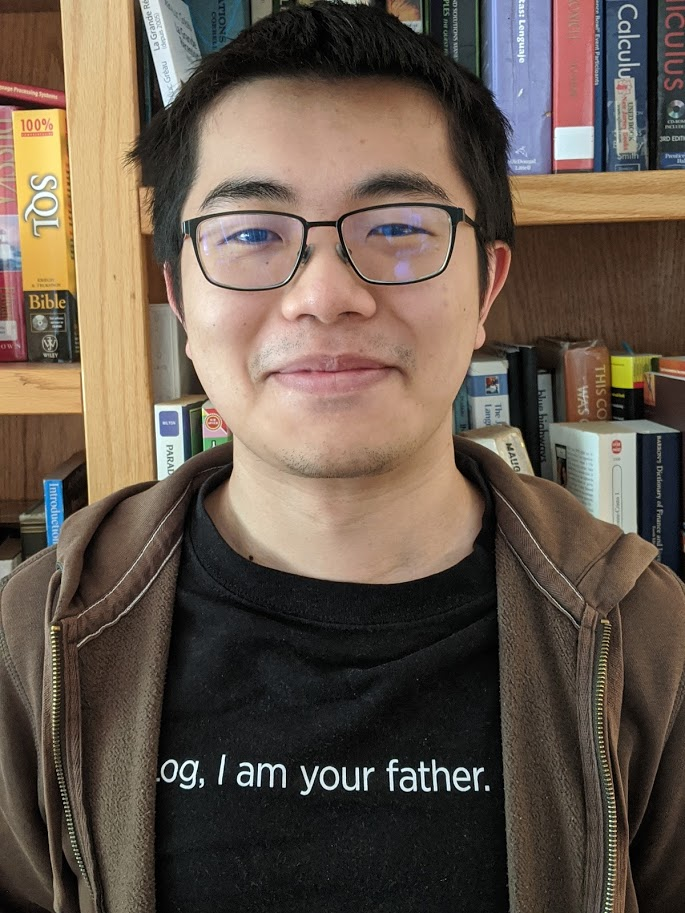
\includegraphics[scale=.25]{mao.jpg}
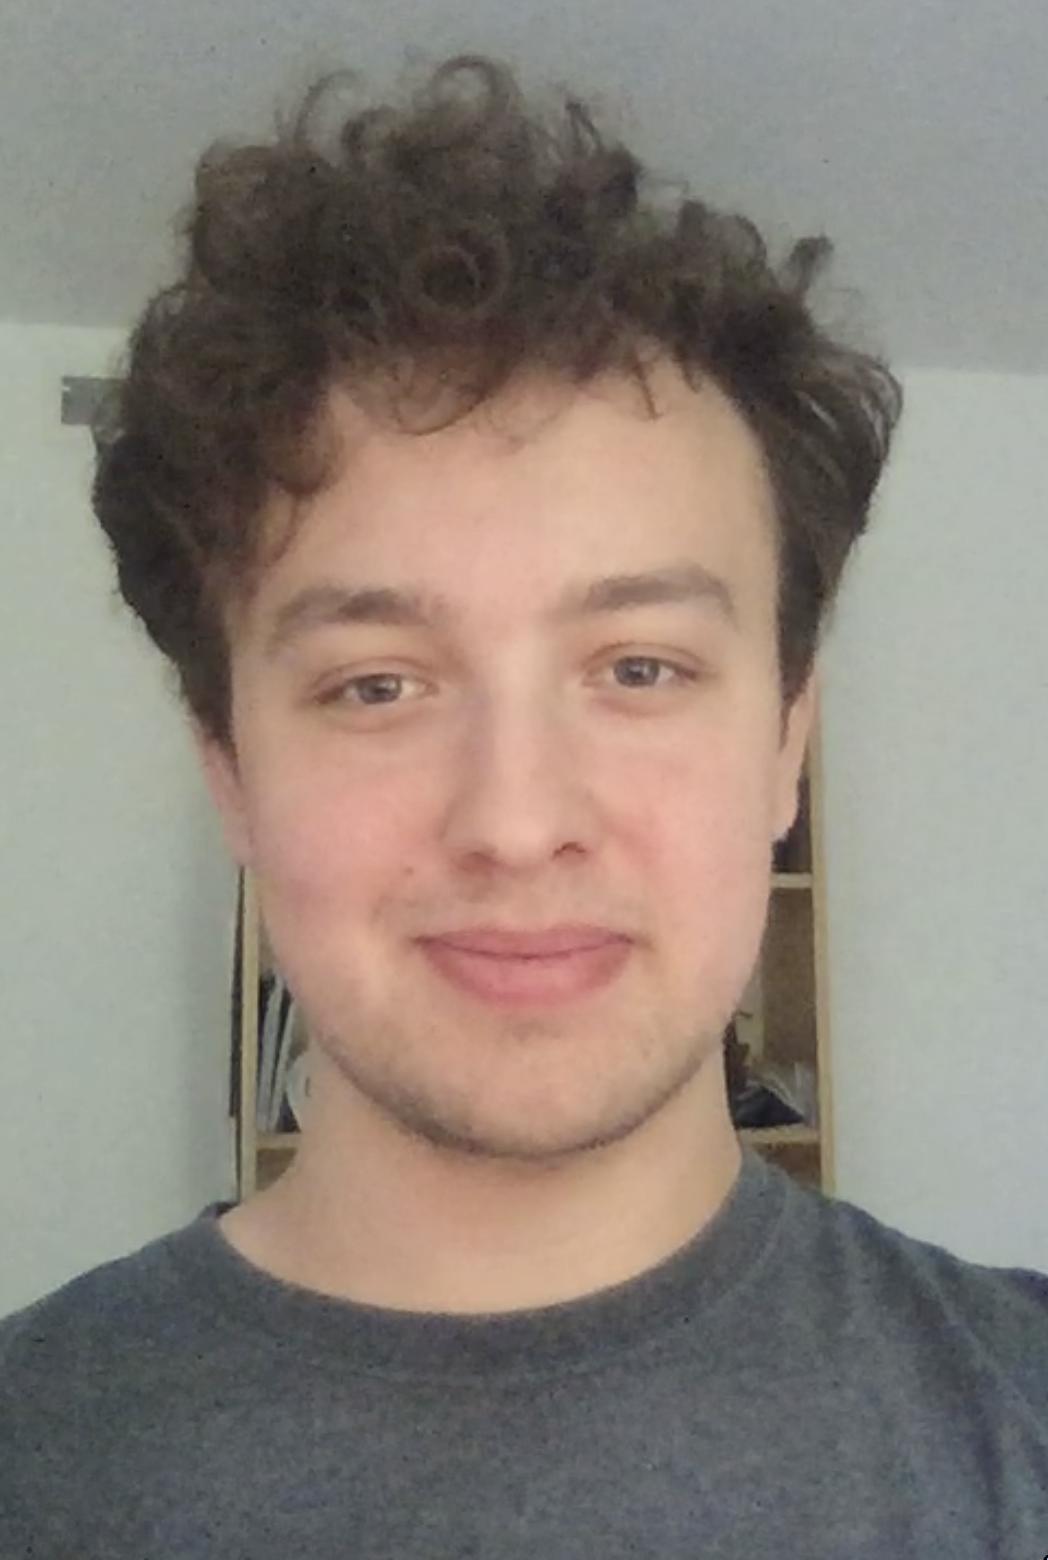
\includegraphics[scale=.293]{Hans.png} % replace with Hans
\end{tabular}
\captionsetup{labelformat=empty}
\caption{The team: Allen to the left, Hans to the right}
\end{figure}
% insert personal bios and anecdotes here:
We are both undergraduate students at the University of California, Berkeley. Allen is a Computer Science major who is primarily interested in Natural Language Processing. Hans is a math and physics major and long time programmer interested in using neural networks to advance the physical and natural sciences. % Allen is CS major at UCB and Hans is math + physics. They met at International House. Little did they know that semester would be so abruptly cut off by a pandemic. (Detail brutal dining conditions at I house.) Shock and horror at news coming in about so much death.
% Video of Costco customer refusing to wear a mask. Customers like this are selfish and endanger other people's safety. Even worse, store employees have to personally go escort the person out--who knows how many people this person could infect in that time period? Better, have a computer analyze people automatically: computers can't get infected with COVID and now store employees aren't putting their lives at risk thanks to selfish bass turds.
% This inspired us to think about creating such a system. 
\subsection{Previous Work on Mask Identification with Computer Vision}
In the past several months, several organizations, for example Didi Chuxing\footnote{https://github.com/didi/maskdetection} and AI Zoo Tech\footnote{https://github.com/AIZOOTech/FaceMaskDetection} have released open-source pre-trained neural network models on multiple platforms (Keras, Tensorflow, and Caffe) that classify faces within a photo or video as mask-wearing or not. Both models perform spectacularly as the Didi model was trained on a dataset of over 200,000 faces while the AIZoo model consists of 24 convolutional layers trained on approximately 8000 images from WIDER Face and MAFA datasets. Accordingly, the Didi model achieves at least 98\% accuracy and the AIZoo model has a 0.896 ROC AUC (\textit{receiver operating characteristic area under the curve}) for face detection and 0.919 ROC AUC for face mask detection, as seen in their curve below.
\begin{center}
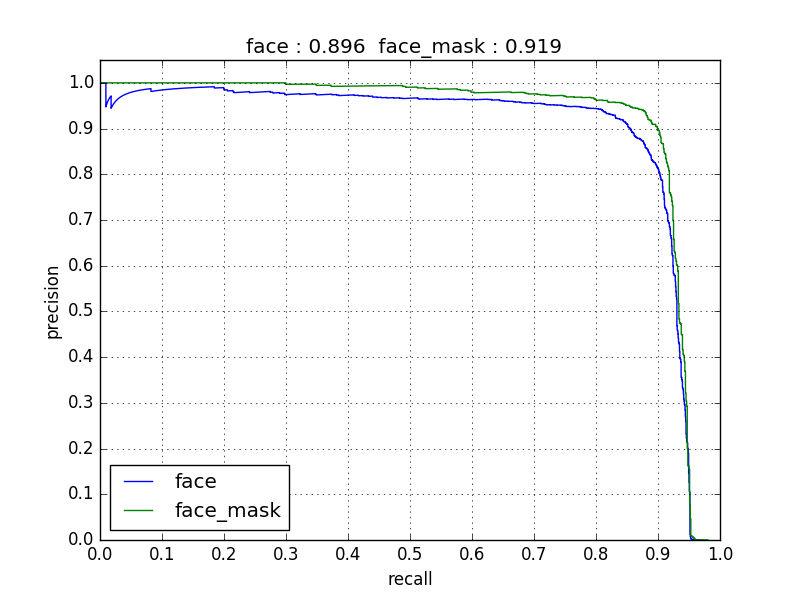
\includegraphics[scale=.5]{pr_curve}
\end{center}


% Computer vision for mask detection
% Computer vision for identifying mask type
\subsection{Our Solution}
Maskit consists of two parts: a Raspberry Pi and a server. We connect a Pi Camera onto the Raspberry Pi such that the Raspberry Pi would be able to take periodic photos. The Raspberry Pi then sends these images to the server via a POST request.
The server then runs the mask detection model on the incoming image and for each face that it identifies, classifies the face as with mask or without mask. These classifications are sent back to the Raspberry Pi as the response to the POST request.
After the Raspberry Pi receives these classifications, if and only if all faces identified wear a mask, then it will activate the servo to open access. In our prototype, we model this situation by raising a welcome flag, though this can be generalized to opening store front doors, for example.
%Google search revealed trained Tensorflow models that recognized human faces. Hans had experience with TF. Allen had experience working with R Pis and servo controls blabla. Combined forces to bring this product together.
%They've come up with prototype that consists of a Rpi and a server. The Rpi is connected to Camera module and servo. It takes pictures at intervals and sends to server as POST request. Server processes pictures with TF model and identifies human faces as masked or unmasked. Then, sends this as response to POST request. If all people identified are wearing a mask, then the raspberry pi activates a welcome flag. Else, people denied entry.
%In model, we have welcome flag, but this can be generalized to any motor, e.g. sliding doors at supermarkets, bolts for regular doors, etc.


\section{Step by Step Usage Instructions}
\subsection{Raspberry Pi Prerequisites}
\subsubsection{Materials}
We used a Raspberry Pi Model B (700-MHz processor, 512 MB RAM). The physical limitations of this Raspberry Pi version are discussed later. In addition to the Raspberry Pi and its regular accessories, i.e. keyboard, power input, etc., we used:
\begin{enumerate}
\item HiTEC HS-5625MG servo \footnote{\url{https://hitecrcd.com/products/servos/sport-servos/digital-sport-servos/hs-5625mg/product}}
\item Pi Camera module \footnote{for setup instructions, see \url{https://www.raspberrypi.org/documentation/usage/camera/}}
\item 6 Volt DC input source. In our case, we put 4 AA batteries into a 9 volt battery case and used aligator clips to join the two empty battery terminals.
\item a breadboard (optional but makes setup nicer)
\end{enumerate}
Our setup should work on the latest version of Raspberry Pi OS (formerly known as \textit{Raspbian}). We will not go in depth on the Raspberry Pi settings on how to enable the Pi Camera or GPIO interfacing (i.e. \texttt{sudo raspi-config}, then enable both GPIO access and camera module), but links are provided in footnotes\footnote{\url{https://www.raspberrypi.org/documentation/configuration/camera.md}}\footnote{\url{https://pimylifeup.com/raspberry-pi-gpio/}}. 

We installed the \texttt{picamera} and \texttt{wiringpi} with \texttt{python pip} for camera and GPIO pin interfacing, respectively, in Python.

In the next section, we describe how to connect the servo to the Raspberry Pi.
\subsubsection{GPIO configuration}
We use the Raspberry Pi's GPIO pins to control the servo. However, the servo cannot draw too much current from the Raspberry Pi without breaking it. As a result, the red servo wire must be connected directly to the 6 volt $V_{in}$. The black servo wire is connected to the ground. Make sure that the Raspberry Pi ground pin is also connected to this ground. The yellow wire is connected to PWM0 (\textit{pulse-width modulation 0}), or physical pin 12\footnote{See \url{https://pinout.xyz/} for Raspberry Pi pin information}.

See below for the Raspberry Pi pinout\footnote{Diagram by \url{https://pinout.xyz/}}:
\begin{center}
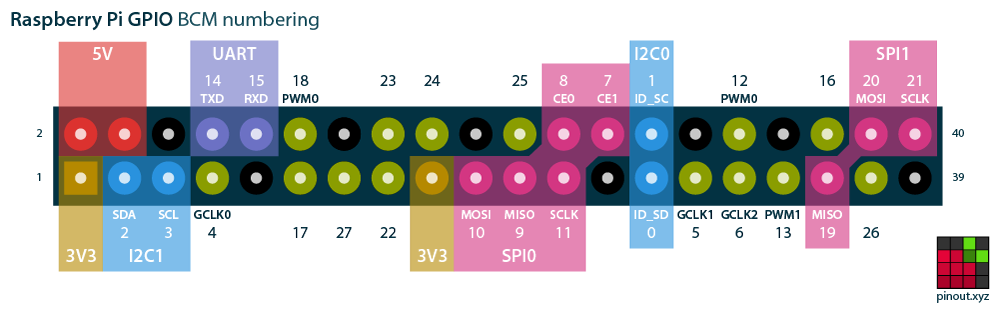
\includegraphics[scale=.5]{raspberry-pi-pinout}
\end{center}

\subsection{Setting up the server}
\begin{enumerate}
\item Install the dependencies found in the \texttt{environment.yml} file\footnote{https://github.com/hansgundlach/FaceMaskDetectionRasPi/blob/master/environment.yml}.
\item On terminal, run \texttt{conda activate maskdetect} to load the environment.
\item Run \texttt{python simple\_server.py}. The server will be hosted on port 8000.
\item The server will now be listening for POST requests.
\item Run \texttt{hostname -I} to get host IP Address. We will need this value in the next step.
\end{enumerate}

\subsection{Running it on R Pi}
To identify the server, the Raspberry Pi must know the server's IP address. In the source  below, the IP address from aboved must be replaced into line 9 below (\texttt{upload\_img\_post.py}).
\lstinputlisting[language=Python]{upload_img_post.py}
After installing other prerequisites (e.g. the \texttt{requests} library\footnote{\url{https://requests.readthedocs.io/en/master/}}), run the client on the Raspberry Pi with the command \texttt{python upload\_img\_post.py}. As the program is currently, the Raspberry Pi takes two images with 5 seconds in between. To adjust this frequency, modify line 22. For perpetual monitoring, it is permissble to add an infinite loop, e.g. \texttt{while True}.

\subsection{A Preview}
We explain a frame from our demonstration video below. The monitor to the left is connected to the Raspberry Pi while the monitor to the right is connected to the desktop. We are displaying video for demonstration purposes; in widescale implementation, both the server and the Raspberry Pi could both be command-line only, i.e. without X-windows. As we see, the server has identified Allen's face as masked and the Raspberry Pi servo has responded accordingly by raising the flag.
\begin{figure}[h!]
\centering
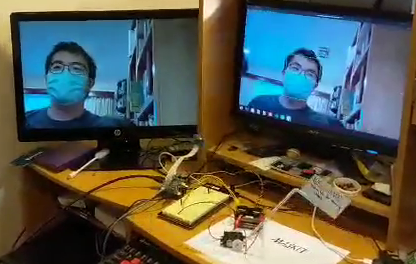
\includegraphics[scale=.5]{cropped}
\captionsetup{labelformat=empty}
\caption{Allen's mask recognized}
\end{figure}

\section{Difficulties and Challenges}
\subsection{Getting Models to Work}
This project was an excellent learning experience for us to learn how to load trained models and use them for interesting applications. We were very fortunate to have found the models by AIZoo (\footnote{\url{https://github.com/AIZOOTech/FaceMaskDetection}}) as these models were not only more or less ready out of the box, but were available on through give of the mainstream deep learning frameworks: PyTorch, TensorFlow, Keras, MXNet, and Caffe. They were in fact not our original attempts as we had initally unsuccessfully tried to compile Didi's models \footnote{\url{https://github.com/didi/maskdetection}}. After that failed, Allen tried to translate some of the C++ code into Python for a better understanding of what was going on, but the short timeline of Hackathons meant that we explored other options and we thus came upon AIZoo's contribution. 
\subsection{Hardware Limitations}
As was mentioned previously, the Raspberry Pi we used is not the latest piece of technology as it contains merely a 700-MHz processor and 512 MB RAM. As such, setup on the Raspberry Pi was time-consuming. Initially, we had ambitions of facial recognition on the Raspberry Pi itself, but this became impossible as loading tensorflow itself would take almost an entire minute; this process would be more of a hindrance to the general public than any help. As such, we devised the server-client system that we have described thus far.

That said, we would be interested in continuing this project with a newer version of the Raspberry Pi, an improvement that would likely significantly boost current performance and perhaps even allow for mask recognition on the Raspberry Pi itself. We discuss these benefits more in depth later.
\subsection{Remote Work}
It goes without saying that work on such a hardware-oriented project is difficult when one teammate lives in Fremont, California and the other in Seattle, Washington. However, now that we have created a working prototype, we are even more proud to have overcome this additional hurdle.
\section{Market Evaluation}
\subsection{Cost Analysis}
As the Raspberry Pi is famous for being a low cost computer, our calculations show that our Raspberry Pi setup can cost even less than \$100, depending on servo quality, a very attractive price to business owners. Prices may be even lower when purchasing from sites such as eBay. Refer to the table below for the cost breakdown:
\begin{table}[h!]
\centering
\begin{tabular}{l|l}
\hline
\multicolumn{1}{|l|}{Item} & \multicolumn{1}{l|}{Cost} \\ \hline
Raspberry Pi               & \$35\footnote{\url{https://www.raspberrypi.org/products/raspberry-pi-4-model-b/}}                      \\
Pi Camera                  & \$29.95\footnote{\url{https://www.adafruit.com/product/3099}}                  \\
Servo                      & \$10-50\footnote{\url{https://www.servocity.com/servos/hitec-servos}}             \\
Batteries and Wiring       & \$10                \\ \hline
Total                      & \$85-125           
\end{tabular}
\end{table}
\subsection{During a Pandemic, Mask Wearing Enforcement is Essential}
The conception for Maskit came actually we watched news reports of customers refusing to wear masks and store employees' safety threatened when forced to deal with these customers \footnote{\url{https://www.youtube.com/watch?v=O8fkVqEZGRA}} and we wondered how we could automatically prevent such unruly customers from entering businesses. Just like how sliding doors at many supermarkets only open when motion detectors are activated, we reasoned that it would be interesting to explore an add-on to this concept, one that integrated facial recognition to open only when the customer wears a mask. 
\section{Suggested Improvements}
\subsection{Additional Features in Public Spaces}
MaskIt needs to be fully evaluated in larger public situations to determine its utility in public spaces. More importantly, we need to implement overrides in case Maskit misidentifies customers with masks as not having a mask. Customers need a contactless way to dispute misidentification. We propose some sort of foot pedal that connects to the Raspberry Pi that the customer can use to dispute a classification. A store attendant on the server side can then make the decision and override Maskit.
\subsection{Image Recognition and Processing on Raspberry Pi}
We hope to invest in newer Raspberry Pis and explore whether it is possible to run the models within the Raspberry Pi alone with comparable efficiency. This form would significantly reduce costs as customers would no longer have to rely on servers.
\subsection{Image Recognition and Processing on the Cloud}
Or the hardware can be made much more streamlined and small and all the image processing can be done on a cloud server instead of a our homemade desktop server. Mask detection can also be done along with other measures to acquire data on COVID-19 symptoms, including temperature detection and heart rate detection. This measurements are effective with just video sources\footnote{\url{https://web.stanford.edu/class/cs231a/prev_projects_2016/finalReport.pdf}}.


\section{Conclusion}
In conclusion, MaskIT has significant potential in research and commercial settings during the COVID pandemic. Given the lack of curret data on mask usage in practice and the importance of mask in the current public health it is important to create automated systems to tack account of mask usage. Some building may need automated gate systems to scan mask usage while universities will need to monitor the percentage of mask compliance on campuses. Systems like MaskIT will be of increasing public importance in the coming months. 

\bibliographystyle{ieeetr}
\bibliography{citations}


\end{document}
